\section{Containerization and Virtualization}
\subsection{Virtualization}
Virtualization is a fundamental concept in modern cloud computing architectures, serving as a resource allocation method that facilitates the delivery of on-demand computing services. It is the process of running a virtual instance of a computer system \cite{Comparison_of_Containerization_and_Virtualization_in_Cloud_Architectures}.

\subsubsection{Mechanism of Virtualization (VMs)}
Hypervisor-based virtualization, which creates Virtual Machines (VMs), works by virtualizing hardware resources to provide the abstraction of an entire computer system. This approach allows multiple operating systems (OSes) to coexist on a single physical machine \cite{Containers_or_Hypervisors_Which_is_Better_for_Database_Consolidation}.

\begin{enumerate}
    \item \textbf{Hypervisors:} Virtualization relies on software known as Hypervisors or Virtual Machine Monitors (VMMs), which run and monitor the VMs \cite{Comparison_of_Containerization_and_Virtualization_in_Cloud_Architectures}.
    \begin{itemize}
        \item \textbf{Type 1 (Bare Metal):} These hypervisors interact directly with the host device’s physical hardware. An example of a Type-1 hypervisor is Xen \cite{Comparison_of_Containerization_and_Virtualization_in_Cloud_Architectures}.

        \item \textbf{Type 2 (Hosted):} These are software applications installed on top of the host operating system, similar to any regular application \cite{Comparison_of_Containerization_and_Virtualization_in_Cloud_Architectures}.
    \end{itemize}

    \begin{figure}[H]
        \centering
        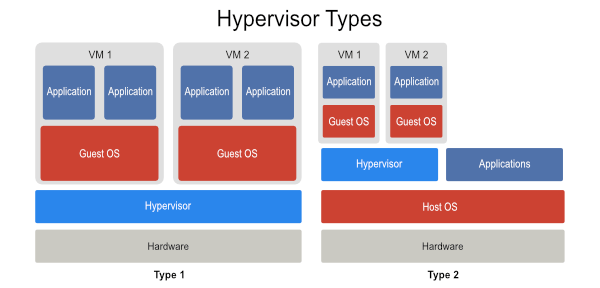
\includegraphics[width=1\linewidth]{images//container/Hypervisor-Types.png}
        \caption{Hypervisor types}
        \label{fig:hypervisor_types}
    \end{figure}

    \item \textbf{Resource Allocation and Isolation:} In this model, a guest OS runs on top of the hypervisor (or host OS in Type 2). Hardware devices are virtualized, often using device emulators \cite{Containers_or_Hypervisors_Which_is_Better_for_Database_Consolidation}. Crucially, each VM is provisioned with a complete, separate operating system \cite{Emerging_Trends_Techniques_and_Open_Issues_of_Containerization_A_Review}.
    \begin{itemize}
        \item \textbf{Strong Isolation:} VMs provide strong performance isolation because they separate the guest operating systems, meaning no data structures in the guest OSes are shared among VMs. This isolation is critical for ensuring that the resource consumption or failure of one VM does not affect other co-located VMs \cite{Emerging_Trends_Techniques_and_Open_Issues_of_Containerization_A_Review}.

        \item \textbf{Resource Overhead:} Because each deployed database or application requires its own full operating system, virtualization often leads to higher resource consumption and larger memory footprints compared to containerization. VMs are known for having slower spin-up/down times, requiring several seconds for booting \cite{Emerging_Trends_Techniques_and_Open_Issues_of_Containerization_A_Review}.
    \end{itemize}
\end{enumerate}


\subsection{Containerization}
Containerization is an alternative resource allocation method and is sometimes referred to as OS-level virtualization or system virtualization in which only the necessary services and packages can be installed on a minimal operating system. These resources are all independent so working with their dependencies and managing them becomes easier. Applications can be abstracted from the environment in which they actually run, which allows container-based applications to be deployed easily and
consistently \cite{Comparison_of_Containerization_and_Virtualization_in_Cloud_Architectures}.

\begin{figure}[H]
    \centering
    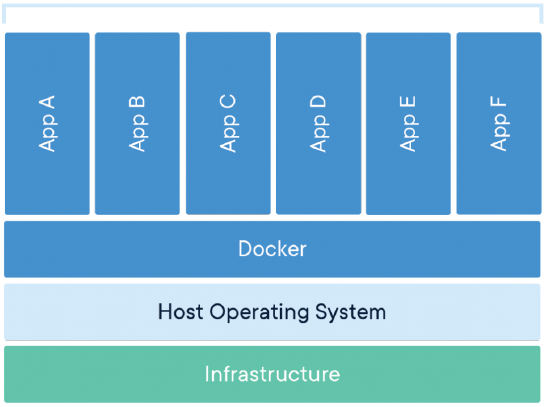
\includegraphics[width=0.85\textwidth]{images//container/container.png}
    \caption{Containerized Environment making use of Docker}
    \label{fig:containerized_environment_docker}
\end{figure}


\subsubsection{Mechanism of Containerization}
\begin{enumerate}
    \item \textbf{Shared Kernel Architecture:} Containers create multiple virtual units in the userspace but, unlike VMs, they share the same host kernel. This inherent sharing is why containers are considered extremely lightweight, as they eliminate the need for running a complete operating system inside each virtual environment \cite{Containers_or_Hypervisors_Which_is_Better_for_Database_Consolidation, Emerging_Trends_Techniques_and_Open_Issues_of_Containerization_A_Review}.

    \item \textbf{Minimal Resources:} In a containerized environment, only the necessary services and packages needed to run a specific application are installed on a minimal operating system. Applications are abstracted from the environment in which they actually run \cite{Comparison_of_Containerization_and_Virtualization_in_Cloud_Architectures, Emerging_Trends_Techniques_and_Open_Issues_of_Containerization_A_Review}.

    \item  \textbf{Isolation Mechanisms:} Containers are isolated from each other through private namespaces (which partition resources to groups of processes) and cgroups (control groups, which manage and limit resources like CPU, memory, and I/O) at the OS level. Namespaces impose instance-specific resource visibility, while cgroups limit the amount of system resources used by an instance \cite{Emerging_Trends_Techniques_and_Open_Issues_of_Containerization_A_Review}.

    \item \textbf{Efficiency:} The design of containerization, exemplified by tools like Docker, aims to overcome the performance overheads associated with VM device emulation and running full guest operating systems. Containers are highly portable, energy and resource efficient, and significantly quick during boot-up, often requiring only a few milliseconds \cite{Containers_or_Hypervisors_Which_is_Better_for_Database_Consolidation, Emerging_Trends_Techniques_and_Open_Issues_of_Containerization_A_Review}.
\end{enumerate}

\subsection{Comparison and Key Differences}
The primary distinction between virtualization (VMs) and containerization lies in the level at which they provide isolation and the degree to which they share the host system's resources:

Containers shift the layer of virtualization from hardware to the OS level, which generally gives them a performance advantage due to negligible virtualization overheads compared to VMs. They are often found to be more efficient in performance for SaaS (Software as a Service) and PaaS (Platform as a Service) offerings \cite{Containers_or_Hypervisors_Which_is_Better_for_Database_Consolidation, Comparison_of_Containerization_and_Virtualization_in_Cloud_Architectures}.

Several studies have analyzed the relationship between containerization, virtualization, and cloud service orchestration. Research shows that the gap between virtualization and containerization is smaller than that in deployment and orchestration, motivating further work. Containers can run on small devices and Linux distributions, while IaaS offers cost savings by offloading infrastructure management. Virtualized applications can be deployed in IaaS environments, and containers are increasingly used in PaaS for fine-grained resource control due to faster startup times and better performance than VMs. Major companies like Amazon, Google, and Facebook provide robust cloud platforms. Technically, virtualization (e.g., KVM) involves separate guest OSs on emulated hardware, whereas containerization (e.g., Docker) runs atop the host OS and provides application-level APIs. In SaaS, tenants operate securely on a shared multi-tenant system as if they have dedicated software instances \cite{Comparison_of_Containerization_and_Virtualization_in_Cloud_Architectures}.

\renewcommand{\arraystretch}{1.5} % 1.0 = default, 1.5 = 50% taller rows
\begin{table}[h]
    \centering
    \begin{tabular}{|>{\raggedright\arraybackslash}p{4cm}|
                     >{\raggedright\arraybackslash}p{4cm}|
                     >{\raggedright\arraybackslash}p{4cm}|}
        \hline
        \textbf{Feature} & \textbf{Virtualization} & \textbf{Containerization} \\ \hline
        Level of Abstraction & Hardware (via Hypervisor) & OS/Kernel (via Namespaces/cgroups) \\ \hline
        Operating System & Each VM runs a full, separate Guest OS & Containers share the single Host OS kernel \\ \hline
        Isolation & Strong (Hardware-level partitioning) & Weaker (OS-level isolation) \\ \hline
        Resource Footprint & Large (due to full OS image) & Small/Lightweight (minimal packages) \\ \hline
        Startup Time & Slower (requires booting OS, several seconds) & Faster (milliseconds) \\ \hline
    \end{tabular}
    \caption{Comparison between containerization and virtualization}
    \label{tab:placeholder}
\end{table}

\subsection{Database Performance}
The study examined four popular relational database management systems: MySQL, PostgreSQL, Microsoft SQL Server, and Oracle. To evaluate performance, the researchers measured the execution times of fundamental database operations, specifically INSERT, UPDATE, DELETE, and SELECT queries. Each test scenario was repeated 100 times across four increasing datasets, with the largest dataset containing 1,000,000 records in the primary table \cite{Performance_analysis_of_databases_created_in_virtualized_and_containerized_environment}.

Two primary hypotheses guided the research:
\begin{enumerate}
    \item H1 assumed that databases running on Docker containers would be more efficient than those on virtual machines.
    \item H2 assumed that Oracle would be the most efficient database regardless of the environment.
\end{enumerate}

The results confirmed the first hypothesis (H1), showing that databases running on Docker containers outperform instances running on virtual machines in terms of performance \cite{Performance_analysis_of_databases_created_in_virtualized_and_containerized_environment}.

However, the findings rejected the second hypothesis (H2). The study found that the PostgreSQL database demonstrated a definite advantage in performance over the other analyzed databases in terms of SQL query execution speed. PostgreSQL consistently achieved the shortest execution times across INSERT, DELETE, and UPDATE scenarios \cite{Performance_analysis_of_databases_created_in_virtualized_and_containerized_environment}.

While containers often outperform VMs in general application deployment speed and resource utilization, the optimal choice for databases, particularly in Database-as-a-Service (DBaaS) environments, is nuanced and depends heavily on the workload characteristics, especially concerning Input/Output (I/O) operations and isolation requirements. The MySQL database obtained comparable results to PostgreSQL, generally showing only slightly longer execution times. In contrast, the Oracle system was typically ranked third or last among the systems tested, depending on the specific scenario, and MS SQL Server often performed the worst, especially with larger datasets in DELETE and UPDATE operations \cite{Performance_analysis_of_databases_created_in_virtualized_and_containerized_environment}.

\begin{figure}[H]
    \centering
    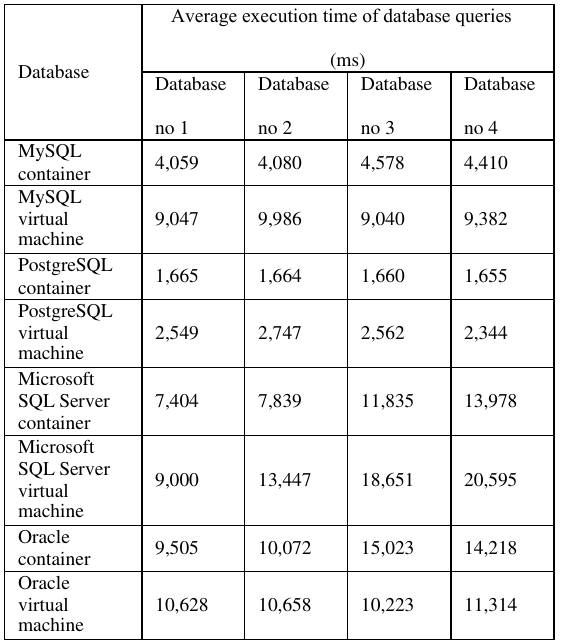
\includegraphics[width=0.7\textwidth]{images//container/_1.png}
    \caption{Average query execution times for the scenario Research Programme No. 1 \cite{Performance_analysis_of_databases_created_in_virtualized_and_containerized_environment}.}
    \label{fig:database_performance1}
\end{figure}

\begin{figure}[H]
    \centering
    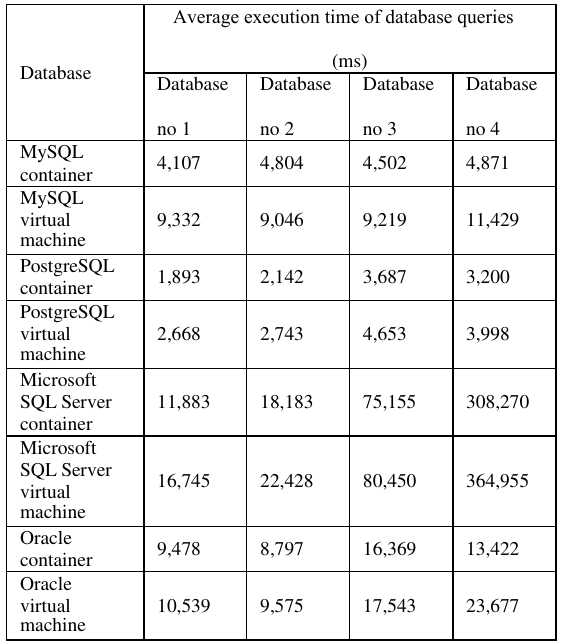
\includegraphics[width=0.7\textwidth]{images//container/_2.png}
    \caption{Average query execution times for the scenario Research Programme No. 2 \cite{Performance_analysis_of_databases_created_in_virtualized_and_containerized_environment}.}
    \label{fig:database_performance2}
\end{figure}

\begin{figure}[H]
    \centering
    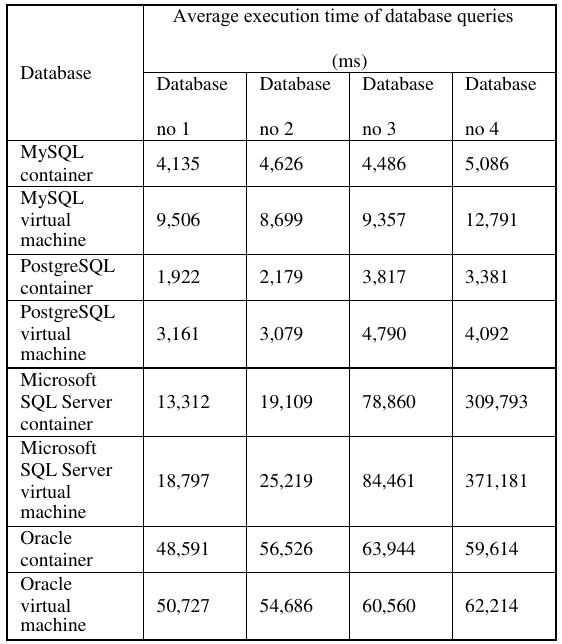
\includegraphics[width=0.7\textwidth]{images//container/_3.png}
    \caption{Average query execution times for the scenario Research Programme No. 3 \cite{Performance_analysis_of_databases_created_in_virtualized_and_containerized_environment}.}
    \label{fig:database_performance3}
\end{figure}

In summary, the research concluded that the containerized environment offers superior performance for relational databases compared to virtualization, and that PostgreSQL currently leads in efficiency among the tested systems \cite{Performance_analysis_of_databases_created_in_virtualized_and_containerized_environment}.



\subsection{Databases and Workload Sensitivity}

Database Management Systems (DBMSs) are a common and critical service in the cloud, where disk I/O performance and performance isolation are crucial. DBMS workloads are typically update-intensive and issue frequent fsync calls to maintain file system consistency, which significantly relies on journaling mechanisms \cite{Containers_or_Hypervisors_Which_is_Better_for_Database_Consolidation}.

\subsubsection{The I/O Performance Anomaly in Containers}

Contrary to the general belief that containers (like LXC) inherently outperform hypervisor-based virtualization (like KVM) due to less overhead, research has shown that for DBMS workloads, KVM often outperforms LXC in both I/O performance and isolation \cite{Containers_or_Hypervisors_Which_is_Better_for_Database_Consolidation}.

Contrary to the common assumption that container-based virtualization offers superior performance due to lower overhead, prior studies indicate that hypervisor-based virtualization (e.g., KVM) can outperform containers (e.g., LXC) for database workloads. This performance discrepancy primarily arises from file system journaling behavior \cite{Containers_or_Hypervisors_Which_is_Better_for_Database_Consolidation}..

In containerized environments, all containers share a single host kernel and a common journaling module, which serializes commit operations across containers. As a result, database workloads may experience increased latency and reduced throughput due to interference from unrelated I/O activities \cite{Containers_or_Hypervisors_Which_is_Better_for_Database_Consolidation}..

In contrast, virtual machines maintain independent file systems and journaling modules, enabling parallel commit operations and minimizing cross-tenant interference. Empirical results demonstrate that KVM can achieve up to 64higher throughput than LXC for MySQL workloads, highlighting its suitability for I/O-intensive DBMS applications \cite{Containers_or_Hypervisors_Which_is_Better_for_Database_Consolidation}.

% \begin{enumerate}
%     \item \textbf{The Journaling Bottleneck:} The primary reason for containers' inferior performance in  database environments is related to file system journaling \cite{Containers_or_Hypervisors_Which_is_Better_for_Database_Consolidation}.
%     \begin{itemize}
%         \item In container environments, only one journaling module is effective because containers share a single host kernel.
        
%         \item This shared journaling module batches updates from multiple containers into transactions and commits them to the disk.
        
%         \item Since transactions are serialized in the journaling module, and a single transaction may contain updates from multiple containers, one container must wait for unrelated data belonging to other containers to be flushed. This serialization creates a bottleneck.
%     \end{itemize}

%     \item \textbf{VM Advantage:} Hypervisor-based virtualization (VMs) avoids this journal-related problem because each VM has its own fully separated file system and its own journaling module, allowing commits to happen in parallel and reducing interference \cite{Containers_or_Hypervisors_Which_is_Better_for_Database_Consolidation}.

%     \item \textbf{Quantified Difference:} In one experiment using a MySQL workload, KVM outperformed LXC in throughput by 64\%. KVM shows superior I/O performance, making it a better fit for hosting DBMS applications that are I/O intensive \cite{Containers_or_Hypervisors_Which_is_Better_for_Database_Consolidation}.
% \end{enumerate}

\subsubsection{Performance Isolation and Resource Guarantee}

For DBaaS, maintaining strong isolation and resource guarantees is mandatory to meet service level agreements.
\begin{enumerate}
    \item \textbf{Weaker Isolation in Containers:} Since containers share kernel data structures and buffer caches at the OS level, performance isolation becomes weaker and harder to achieve. The journaling issue further compounds this; I/O requests originating from the journaling module run outside the container's control group (cgroup) and are not accurately accounted for the container that initiated the commits. As a result, containers may violate resource limits imposed by cgroups \cite{Containers_or_Hypervisors_Which_is_Better_for_Database_Consolidation}.

    \item \textbf{VM Isolation for DBaaS:} VMs provide strong isolation because they run separate guest OSes \cite{Containers_or_Hypervisors_Which_is_Better_for_Database_Consolidation}. Resource reservation within a multi-tenant database context, such as Microsoft SQL Azure, is crucial for performance isolation, ensuring that one tenant's workload is unaffected by co-located tenants \cite{Performance_Isolation_in_MultTenant_Relational_Database_as_a_Service}
\end{enumerate}

\subsection{Conclusion on Database Suitability}
For high-performance, mission-critical, and highly consolidated Database-as-a-Service (DBaaS) environments where disk I/O and strict performance isolation (SLAs) are paramount, virtualization (VMs) is typically the better-suited choice. This is due to the fundamental architecture: VMs offer stronger performance isolation and bypass the bottleneck created by the shared journaling mechanism inherent in OS-level virtualization \cite{Emerging_Trends_Techniques_and_Open_Issues_of_Containerization_A_Review}. 

However, if the priority is fast deployment, efficient resource utilization, and lighter overheads for platforms like PaaS that can tolerate the shared I/O stack, containers are often preferred \cite{Comparison_of_Containerization_and_Virtualization_in_Cloud_Architectures}.

The overall trend seen in the market is that virtualized environments are better suited for IaaS (Infrastructure as a Service) infrastructures, where robustness is valued highly, while containers are found to be efficient for PaaS and SaaS offerings \cite{Comparison_of_Containerization_and_Virtualization_in_Cloud_Architectures}.